%%%%% Document Setup %%%%%%%%

\documentclass[10pt, twocolumn]{revtex4}    % Font size (10,11 or 12pt) and column number (one or two).

\usepackage{times}                          % Times New Roman font type

\usepackage[a4paper, left=1.85cm, right=1.85cm,
 top=1.85cm, bottom=1.85cm]{geometry}       % Defines paper size and margin length

\usepackage[font=small,
labelfont=bf]{caption}                      % Defines caption font size as 9pt and caption title bolded
\captionsetup{justification=raggedright, singlelinecheck=false}

\usepackage{mathtools,amssymb}
\usepackage{graphics,graphicx,epsfig,ulem}	% Makes sure all graphics works
\usepackage{amsmath} 						% Adds mathematical features for equations
\usepackage{siunitx}
\usepackage{textcomp}
\usepackage{enumitem}
\usepackage{bm}
\usepackage{lipsum}
\usepackage[toc,page]{appendix}
\usepackage{booktabs}
\usepackage{rotating}
\usepackage{siunitx}
\usepackage{multirow}
\usepackage{ulem}
\usepackage{array}
\newcolumntype{L}[1]{>{\raggedright\arraybackslash}p{#1}}

\usepackage{etoolbox}                       % Customise date to preferred format
\makeatletter
\patchcmd{\frontmatter@RRAP@format}{(}{}{}{}
\patchcmd{\frontmatter@RRAP@format}{)}{}{}{}
\renewcommand\Dated@name{}
\newcommand{\rom}[1]{\uppercase\expandafter{\romannumeral #1\relax}}
\makeatother

%\usepackage[flushleft]{threeparttable}

\usepackage{fancyhdr}

\pagestyle{fancy}                           % Insert header
\renewcommand{\headrulewidth}{0pt}
\lhead{P. Einarsson Nielsen}                          % Your name
\rhead{TITLE}           % Your report title               

\def\bibsection{\section*{References}}        % Position refernce section correctly


\AtBeginDocument{
	\heavyrulewidth=.08em
	\lightrulewidth=.05em
	\cmidrulewidth=.03em
	\belowrulesep=.65ex
	\belowbottomsep=0pt
	\aboverulesep=.4ex
	\abovetopsep=0pt
	\cmidrulesep=\doublerulesep
	\cmidrulekern=.5em
	\defaultaddspace=.5em
}
\renewcommand{\arraystretch}{1.2}


%%%%% Document %%%%%
\begin{document}                     


\title{TITLE} 
\date{Submitted: \today{}}
\author{P. Einarsson Nielsen}
\affiliation{\normalfont Affiliation}

\begin{abstract}
	\lipsum[1]

\end{abstract}

\maketitle
\thispagestyle{plain} % produces page number for front page



\section{Introduction} \label{s:intro}

The Monte Carlo (MC) method of calculating thermodynamic properties has been well established since originally developed and applied on hard disks. It has had wide reaching impacts on sectors ranging from its intended purpose to computational biology and finance. The Monte Carlo method allows for computer simulations of systems, often under conditions which would be very complex or costly to perform experimentally. This makes it a very versatile tool for obtaining essentially microscopically exact results on various systems. Computer simulations also allow us to wholly determine the method by which particles interact. In this work we investigate three-dimensional spheres interacting by the Lennard-Jones (LJ) potential in an NVT ensemble, where the number of particles, volume and temperature are kept constant. Throughout this work we will use reduced units for distances, temperatures and densities ($\rho{}=N/V$ is number density):
\begin{displaymath}
r^{*} = r/\sigma{},
\end{displaymath}
\begin{displaymath}
T^{*} = k_\text{B}T/\epsilon{},
\end{displaymath}
\begin{displaymath}
\rho{}^{*} = \rho{}\sigma{}^{3} = (N/V)\sigma{}^{3}.
\end{displaymath}
where $\sigma{}$ is the finite distance at which the LJ potential evaluates to zero and $\epsilon{}$ is the depth of the potential well. We take $\sigma=\num{3.4e10}$m and $\epsilon=\num{1.65e21}$J \textbf{reference argon values}. In its reduced form, the LJ potential between two particles can be expressed as
\begin{equation}
U_{LJ}(r^{*}) = 4\left[\left(\frac{1}{r^{*}}\right)^{12}-\left(\frac{1}{r^{*}}\right)^{6}\right]
\end{equation}
where $r^{*}$ is the separation of the two particles.
We perform these simulations for a number of initial configurations, varying the density and temperature of the system.


\section{Methodology} \label{s:methods}
We simulated systems of $N=1000$ particles interacting with the LJ potential. The particles were initialised in a face-centred cubic (FCC) lattice within a cubic container of volume $V$. Conventional boundary conditions, where a particle which moves beyond the boundary of its container is moved to the opposite side, were applied.
MC involves applying a random Cartesian move to each particle in turn, described by
\begin{displaymath}
\Delta{}\bar{s} = d\left(\bar{\xi}-0.5\right)
\end{displaymath}
where $\bar{s}$ and $\bar{\xi}$ are three-vectors containing the move and random numbers between 0 and 1 respectively and $d$ is the maximum displacement.
A move was accepted if it resulted in a decrease in the total potential energy of the system. If not, the move was accepted with a probability proportional to the Boltzmann factor of the resulting state,
\begin{displaymath}
\exp{\frac{\Delta{}U}{k_\text{B}T}}.
\end{displaymath}
where $\Delta{}U, k_\text{B}, T$ are the change in potential energy, Boltzmann constant and system temperature respectively.
This over-weights rarer configurations and is known as importance sampling. At equilibrium, each move is reversible by a move in the opposite direction and, as such, this algorithm satisfies detail balance.
The system was equilibrated over a number, $N_\text{equil}$, of moves such that the initial FCC structure is not present. The maximum displacement, $d$ is adjusted periodically during this equilibration such that the 30-50\% of moves were accepted.
The system was then evolved over further number, $N_\text{evolve}$, of moves and its configuration sampled every periodically. The radial distribution function, $g(r)$, was then calculated and averaged over each particle. The radial distribution function tells us the probability, relative to the ideal gas case, of finding a molecule at a given distance from a reference particle and can be expressed as
\begin{displaymath}
g(r) = \frac{n(r)}{n_\text{ideal}(r)}
\end{displaymath}
where $n_\text{ideal} = \rho{}4\pi{}r^{2}\Delta{}r$, $n(r)$ is the number of particles within a shell of thickness $\Delta{}r$ at a distance $r$, $\rho{}$ is the number density of the system. \textbf{standard long range corrections}

System properties relating to its configuration can be computed from $g(r)$. We compute the excess internal energy per particle by the energy equation \ref{eq:energy} and the excess pressure of the system by the virial equation \ref{eq:pressure}.
\begin{equation}
u^{*} = 2\pi{}\rho{}\int_{0}^{\inf}U_\text{LJ}(r^{*})g(r^{*})(r^{*})^{2}dr^{*}
\label{eq:energy}
\end{equation}
\begin{equation}
p^{*} = P - \rho{}k_\text{B}T = - \frac{2\pi}{3}\rho{}^{2} \int_{0}^{\inf}\frac{U_\text{LJ}(r^{*})}{dr^{*}}g(r^{*})(r^{*})^{3}dr^{*}
\label{eq:pressure}
\end{equation}
In practise the integrals in equations \ref{eq:energy} and \ref{eq:pressure} were approximated as Riemann sums with $dr^{*} \rightarrow{} \Delta{}r^{*} = 0.02$, calculated up to a maximum distance of $r_\text{max}^{*}=6$. The choice of these is discussed in section \ref{ss:numerical}. \textbf{ensure rmax=6 is discussed somewhere}

Each system discussed within was equilibrated over $N_\text{equil}=\num{2e7}$ moves, evolved over $N_\text{evolve}=\num{2e7}$ moves and the configuration sampled every \num{2000} moves.



\section{Results \& Discussion} \label{s:results}
%\lipsum[1-10]

%\textit{The resulting excess energy per particle and excess pressure as functions of the reduced density are shown in figures \ref{fig:excessEnergy} and \ref{fig:excessPressure} respectively. Configuration energy can be seen to reduce from approximately $0$ at $\rho{}^*=0$ before reaching some local minimum value and increasing. The value of $\rho{}^*$ at which this local minima is reached appears to vary as a function of the system temperature; the absolute value of the minima is decreased and occurs at smaller $\rho{}^*$ at higher temperatures when compared to that of lower temperatures.
%Interpretation - at lower densities we are essentially considering an ideal gas; compare to total energy u-config + u-kinetic
%Reduced pressure can be seen to increase *exponentially* from approximately $0$ at $\rho{}^*=0$ with increasing $\rho{}^*$. The rate of increase can be seen to be greater at higher than lower temperatures.
%At very low $\rho{}^*$ the system temperature is observed to have little impact on the configuration energy or pressure. However at larger $\rho{}^*$ the difference between systems of different temperatures increases.}


\subsection{Thermodynamic quantities} \label{ss:thermodynamics}
\begin{figure}
	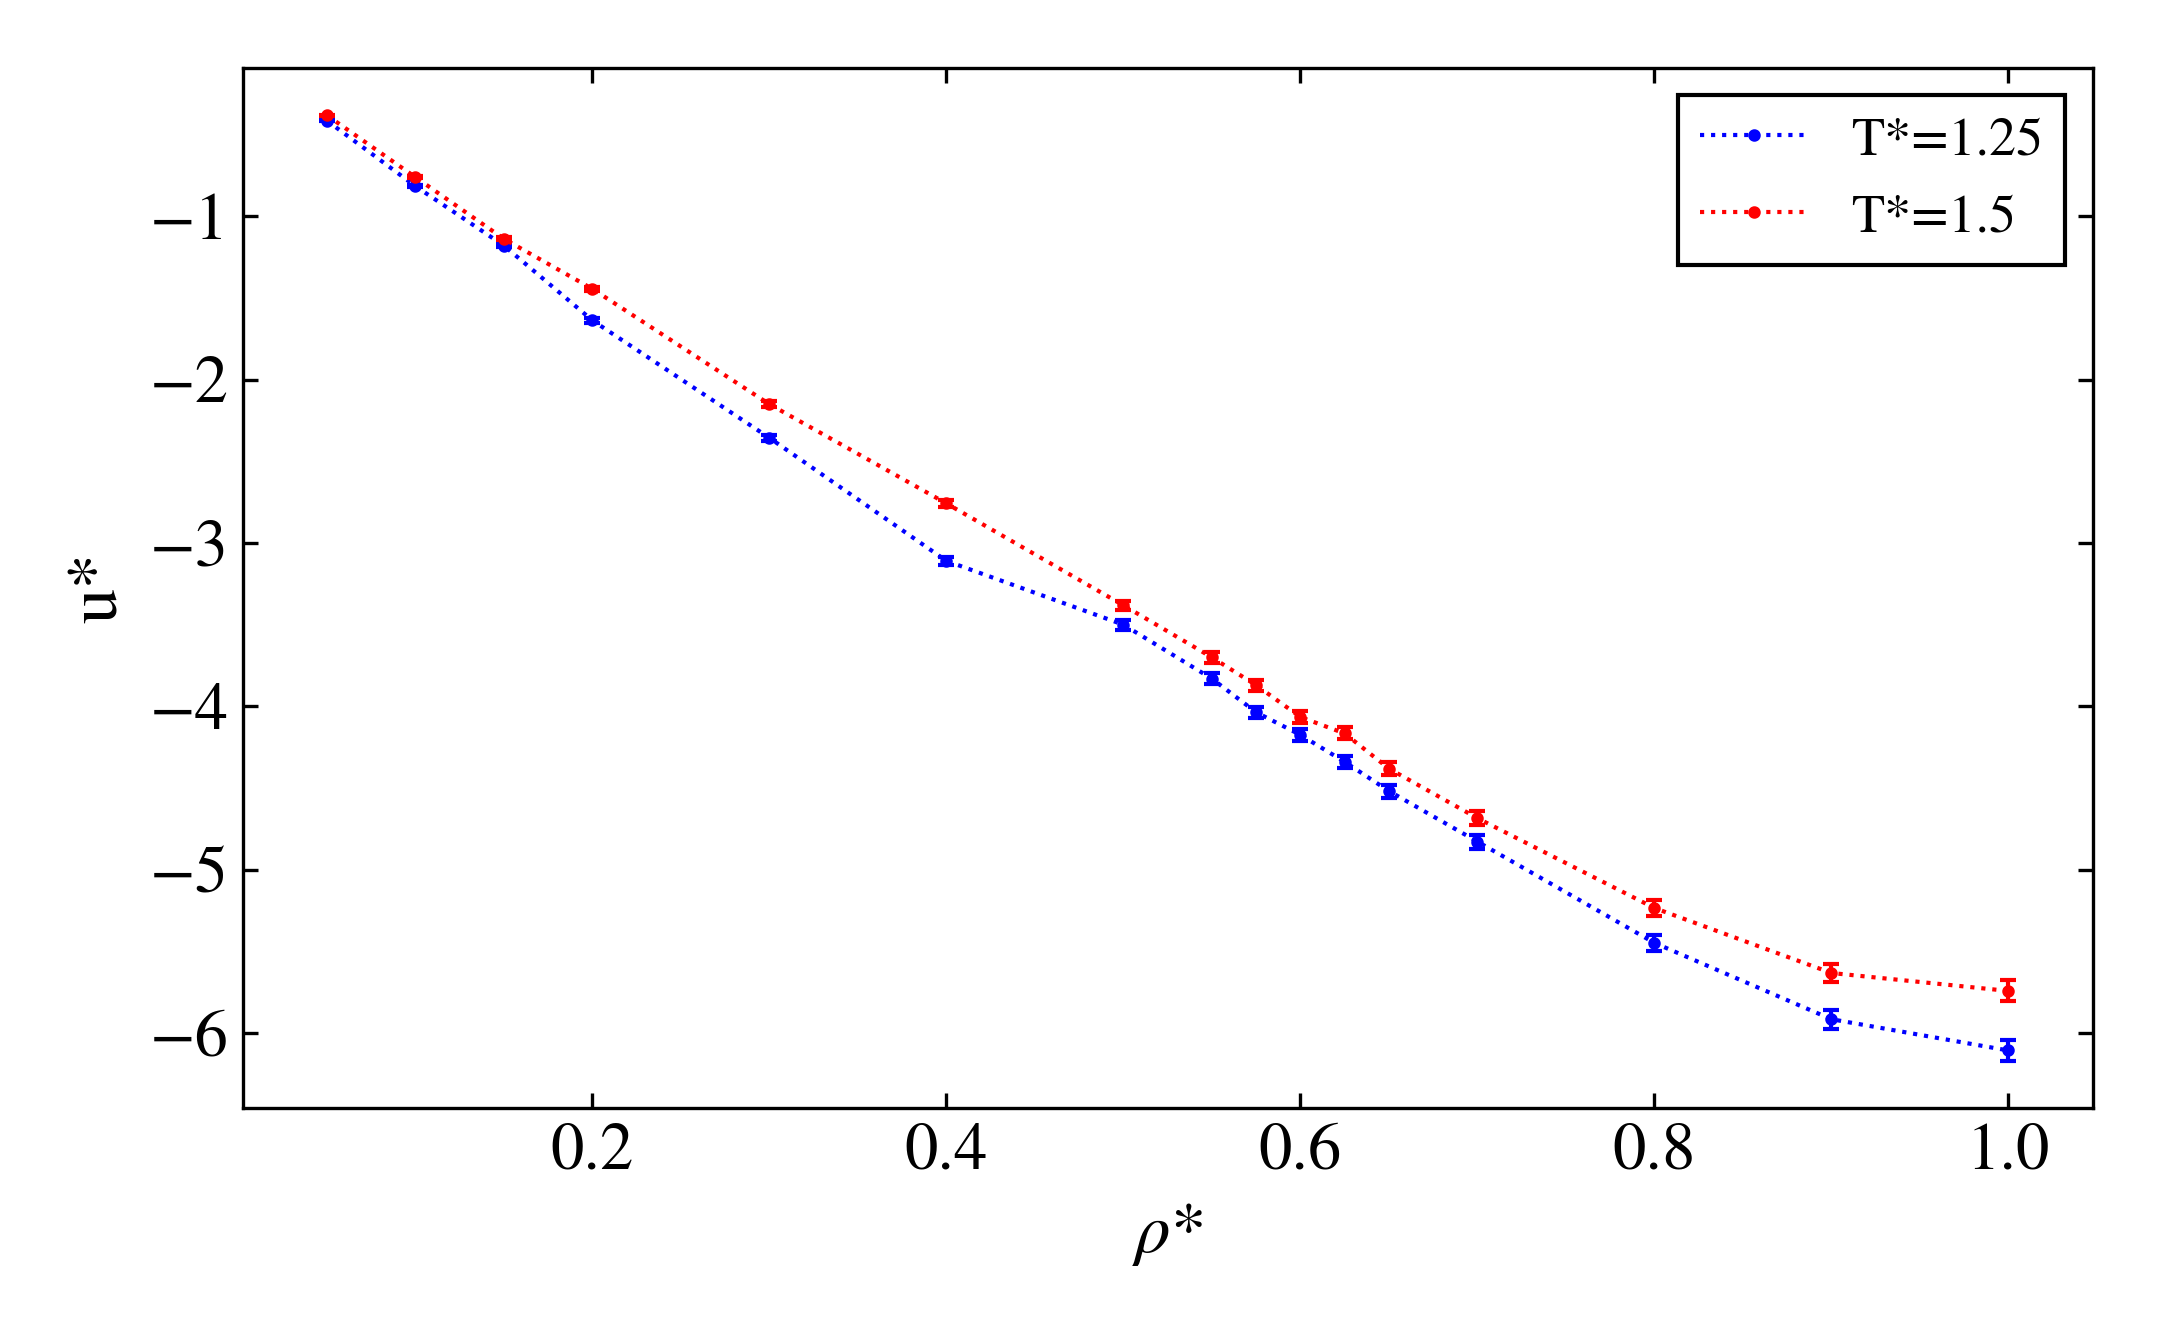
\includegraphics[width=\linewidth]{figures/excessEnergyPressure/excessEnergy.png}
	\caption{MC results for the excess energy per particle, $u^{*}$, against density, $\rho{}^{*}$ along four isotherms $T^{*}=0.75, 1.00, 1.25, 1.50$, each represented by a colour ranging from blue to red. Error bars show the standard error of the mean. Dotted lines have been added to guide the eye.}
	\label{fig:excessEnergy}
\end{figure}
	
\begin{figure}
	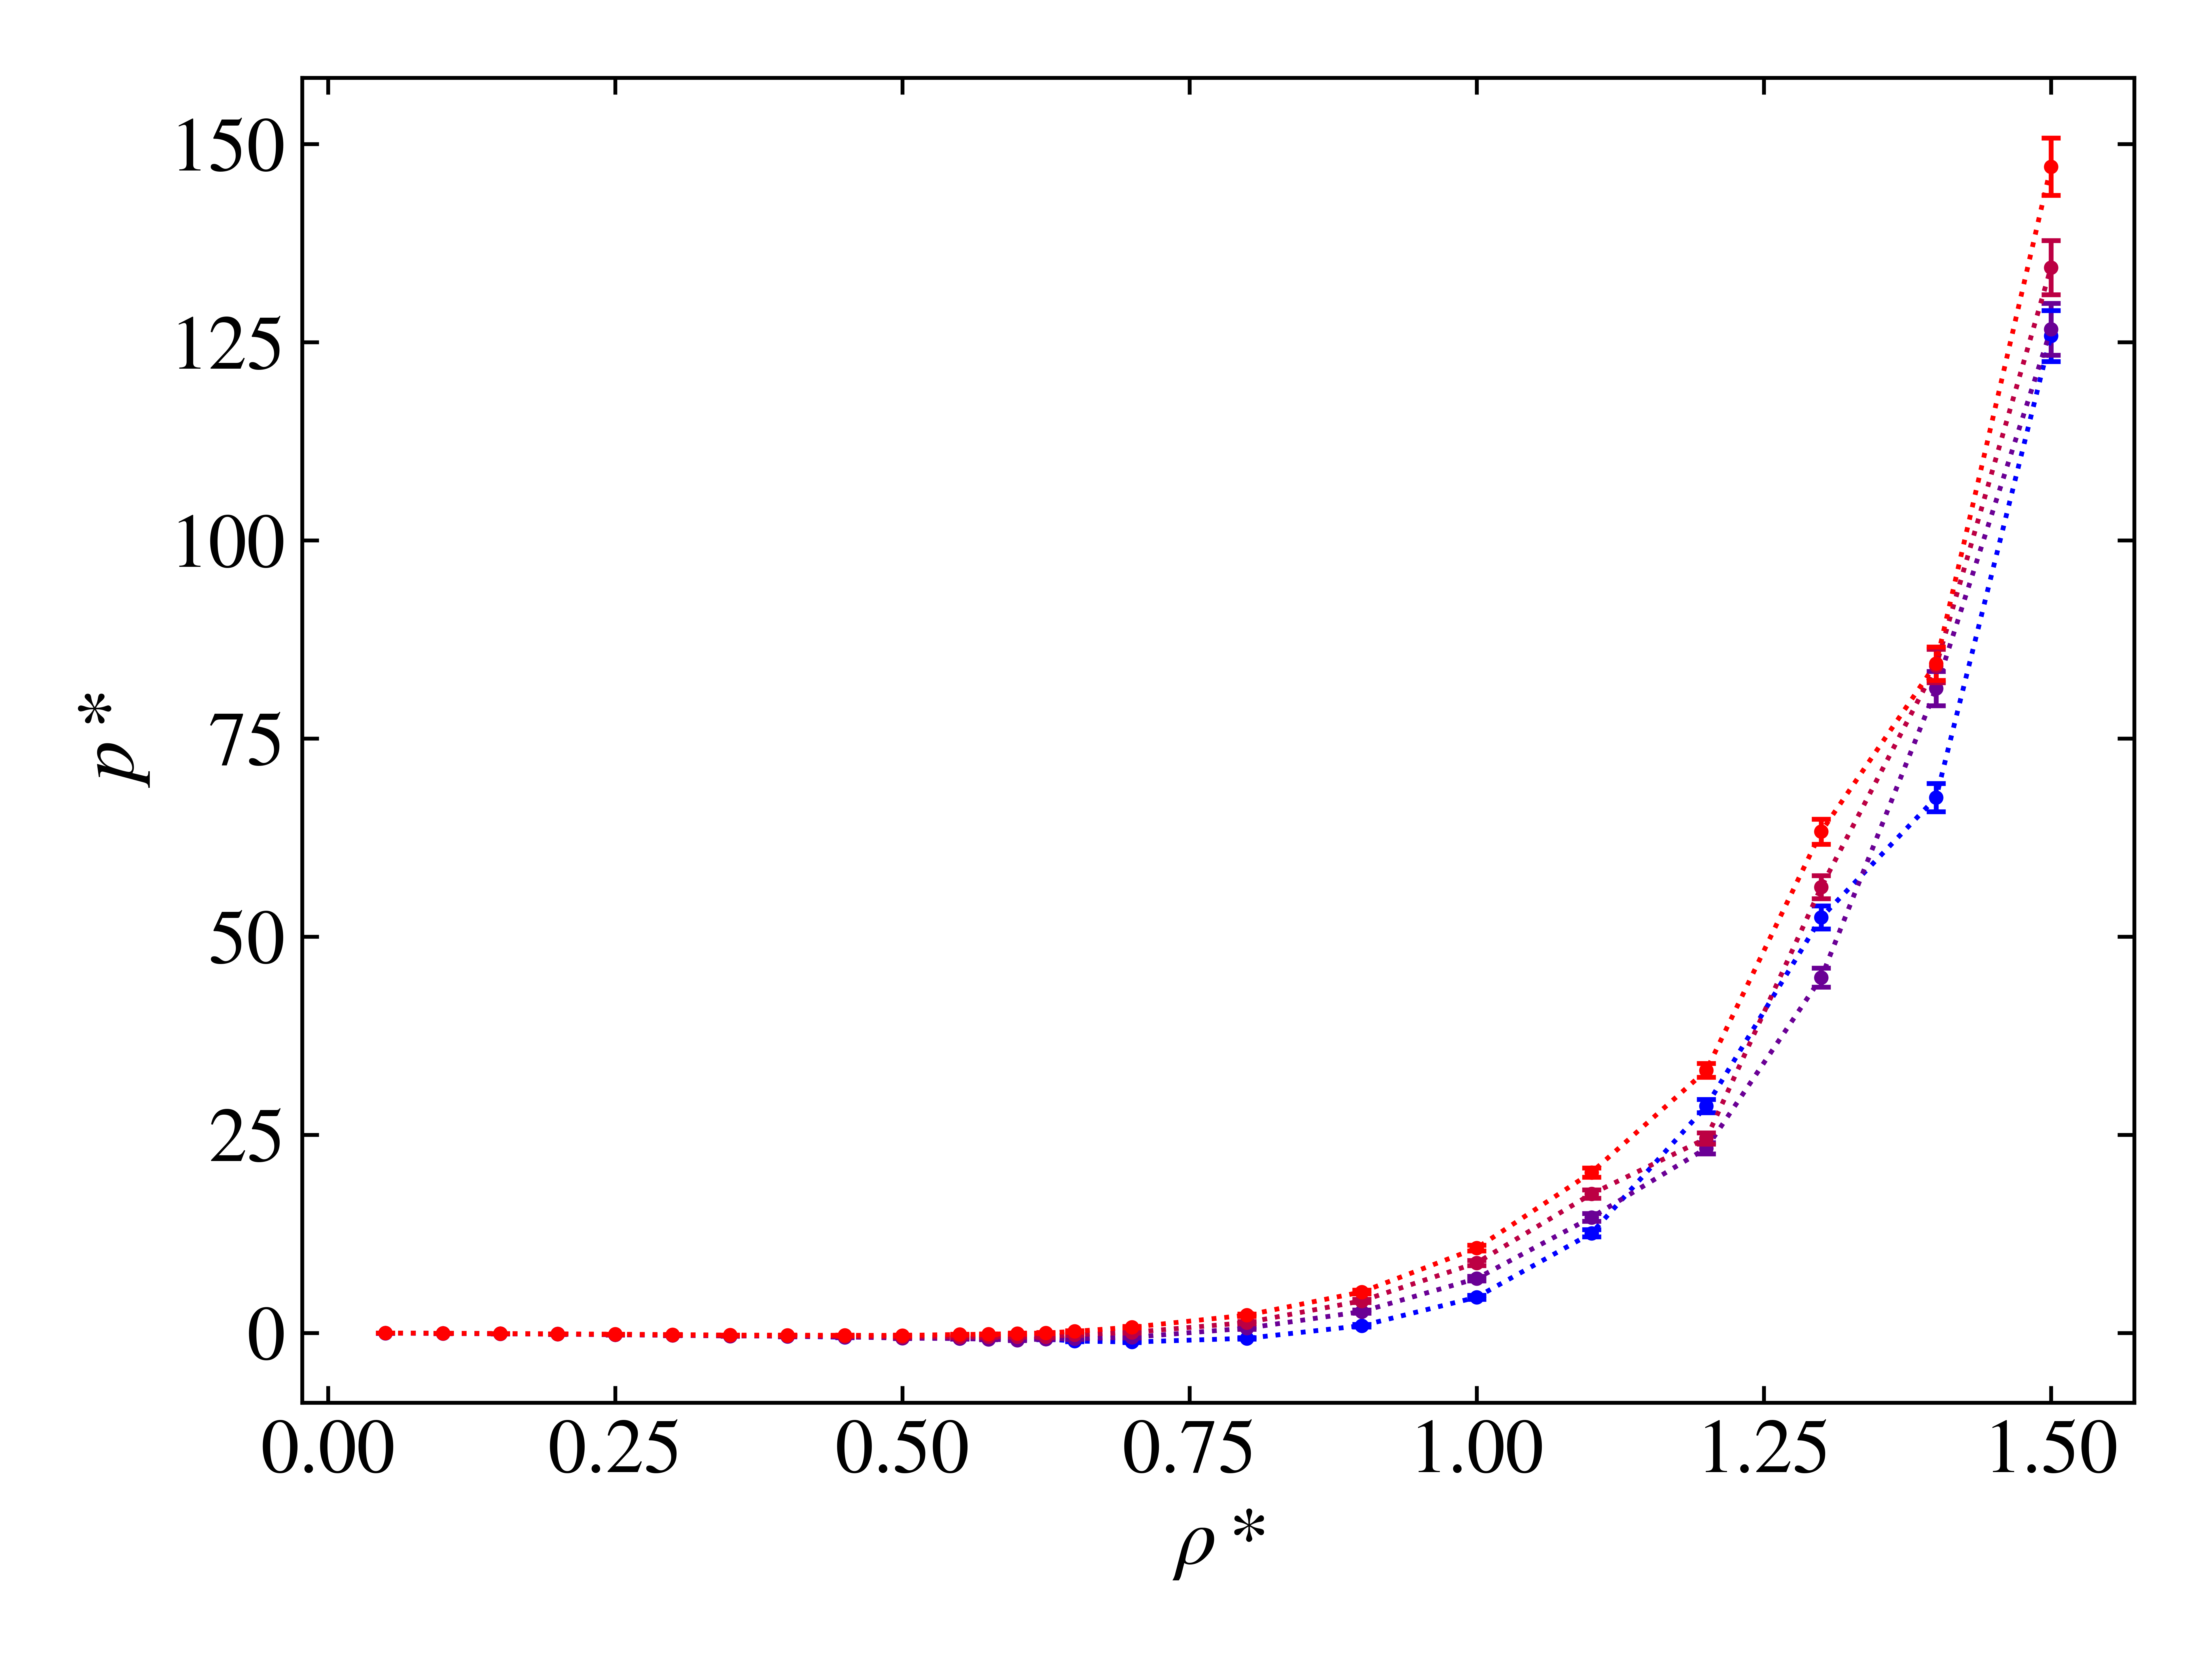
\includegraphics[width=\linewidth]{figures/excessEnergyPressure/excessPressure.png}
	\caption{MC results for the excess pressure, $p^{*}$, against density, $\rho{}^{*}$ along four isotherms $T^{*}=0.75, 1.00, 1.25, 1.50$, each represented by a colour ranging from blue to red. Error bars show the standard error of the mean. Dotted lines have been added to guide the eye.}
	\label{fig:excessPressure}
\end{figure}

%\textit{Typical radial distribution functions for the gaseous, liquid and crystalline solid states are presented in figure \ref{fig:RDFs}. [For each state we observe the RDF to be zero until almost $r^{*}=1$. This is due to the sharp increase in the LJ potential when $r^{*}<1$ and as such these are energetically unfavourable positions for particles to be in close to but less than $r^{*}=1$ and essentially prohibited at $r^{*}<<1$.] A sharp peak is observed at $r^{*}=1$ for each state, beyond which they become distinct. In the gaseous state, $g(r)$ quickly drops to unity beyond $r^{*}=1$, [indicating that the substance is entirely homogeneous and completely lacks order.] In the liquid state, $g(r)$ displays damped oscillatory behaviour beyond $r^{*}=1$, converging to $g(r)=1$ [shortly]. The oscillations in $g(r)$ indicate that at some points we are more or less likely to observe a particle at a given distance from a reference particle [but only up to some medium value beyond which the substance is homogeneous], i.e. short-range order is observed. In the crystalline solid state the formation of many irregular peaks and troughs in $g(r)$, indicating that we are very likely or unlikely to find particles in certain positions. This irregularity is observed over a longer distance than the oscillatory behaviour in the liquid state, indicating the presence of long-range order.}

\begin{figure}
	\includegraphics[width=\linewidth]{figures/rdfs/RDFs.png}
	\caption{Radial distribution functions (RDFs), $g(r^{*})$ of our MC systems along an isotherm $T^{*}=1.5$ at densities $\rho{}^{*}=0.1, 0.8, 1.5$ shown in the lower, middle, upper panel respectively. These typically correspond to vapour-like, liquid-like, solid-like states respectively. Markers are omitted for visual clarity.}
	\label{fig:RDFs}
\end{figure}

\subsection{Numerical methods} \label{ss:numerical}

\begin{figure}
	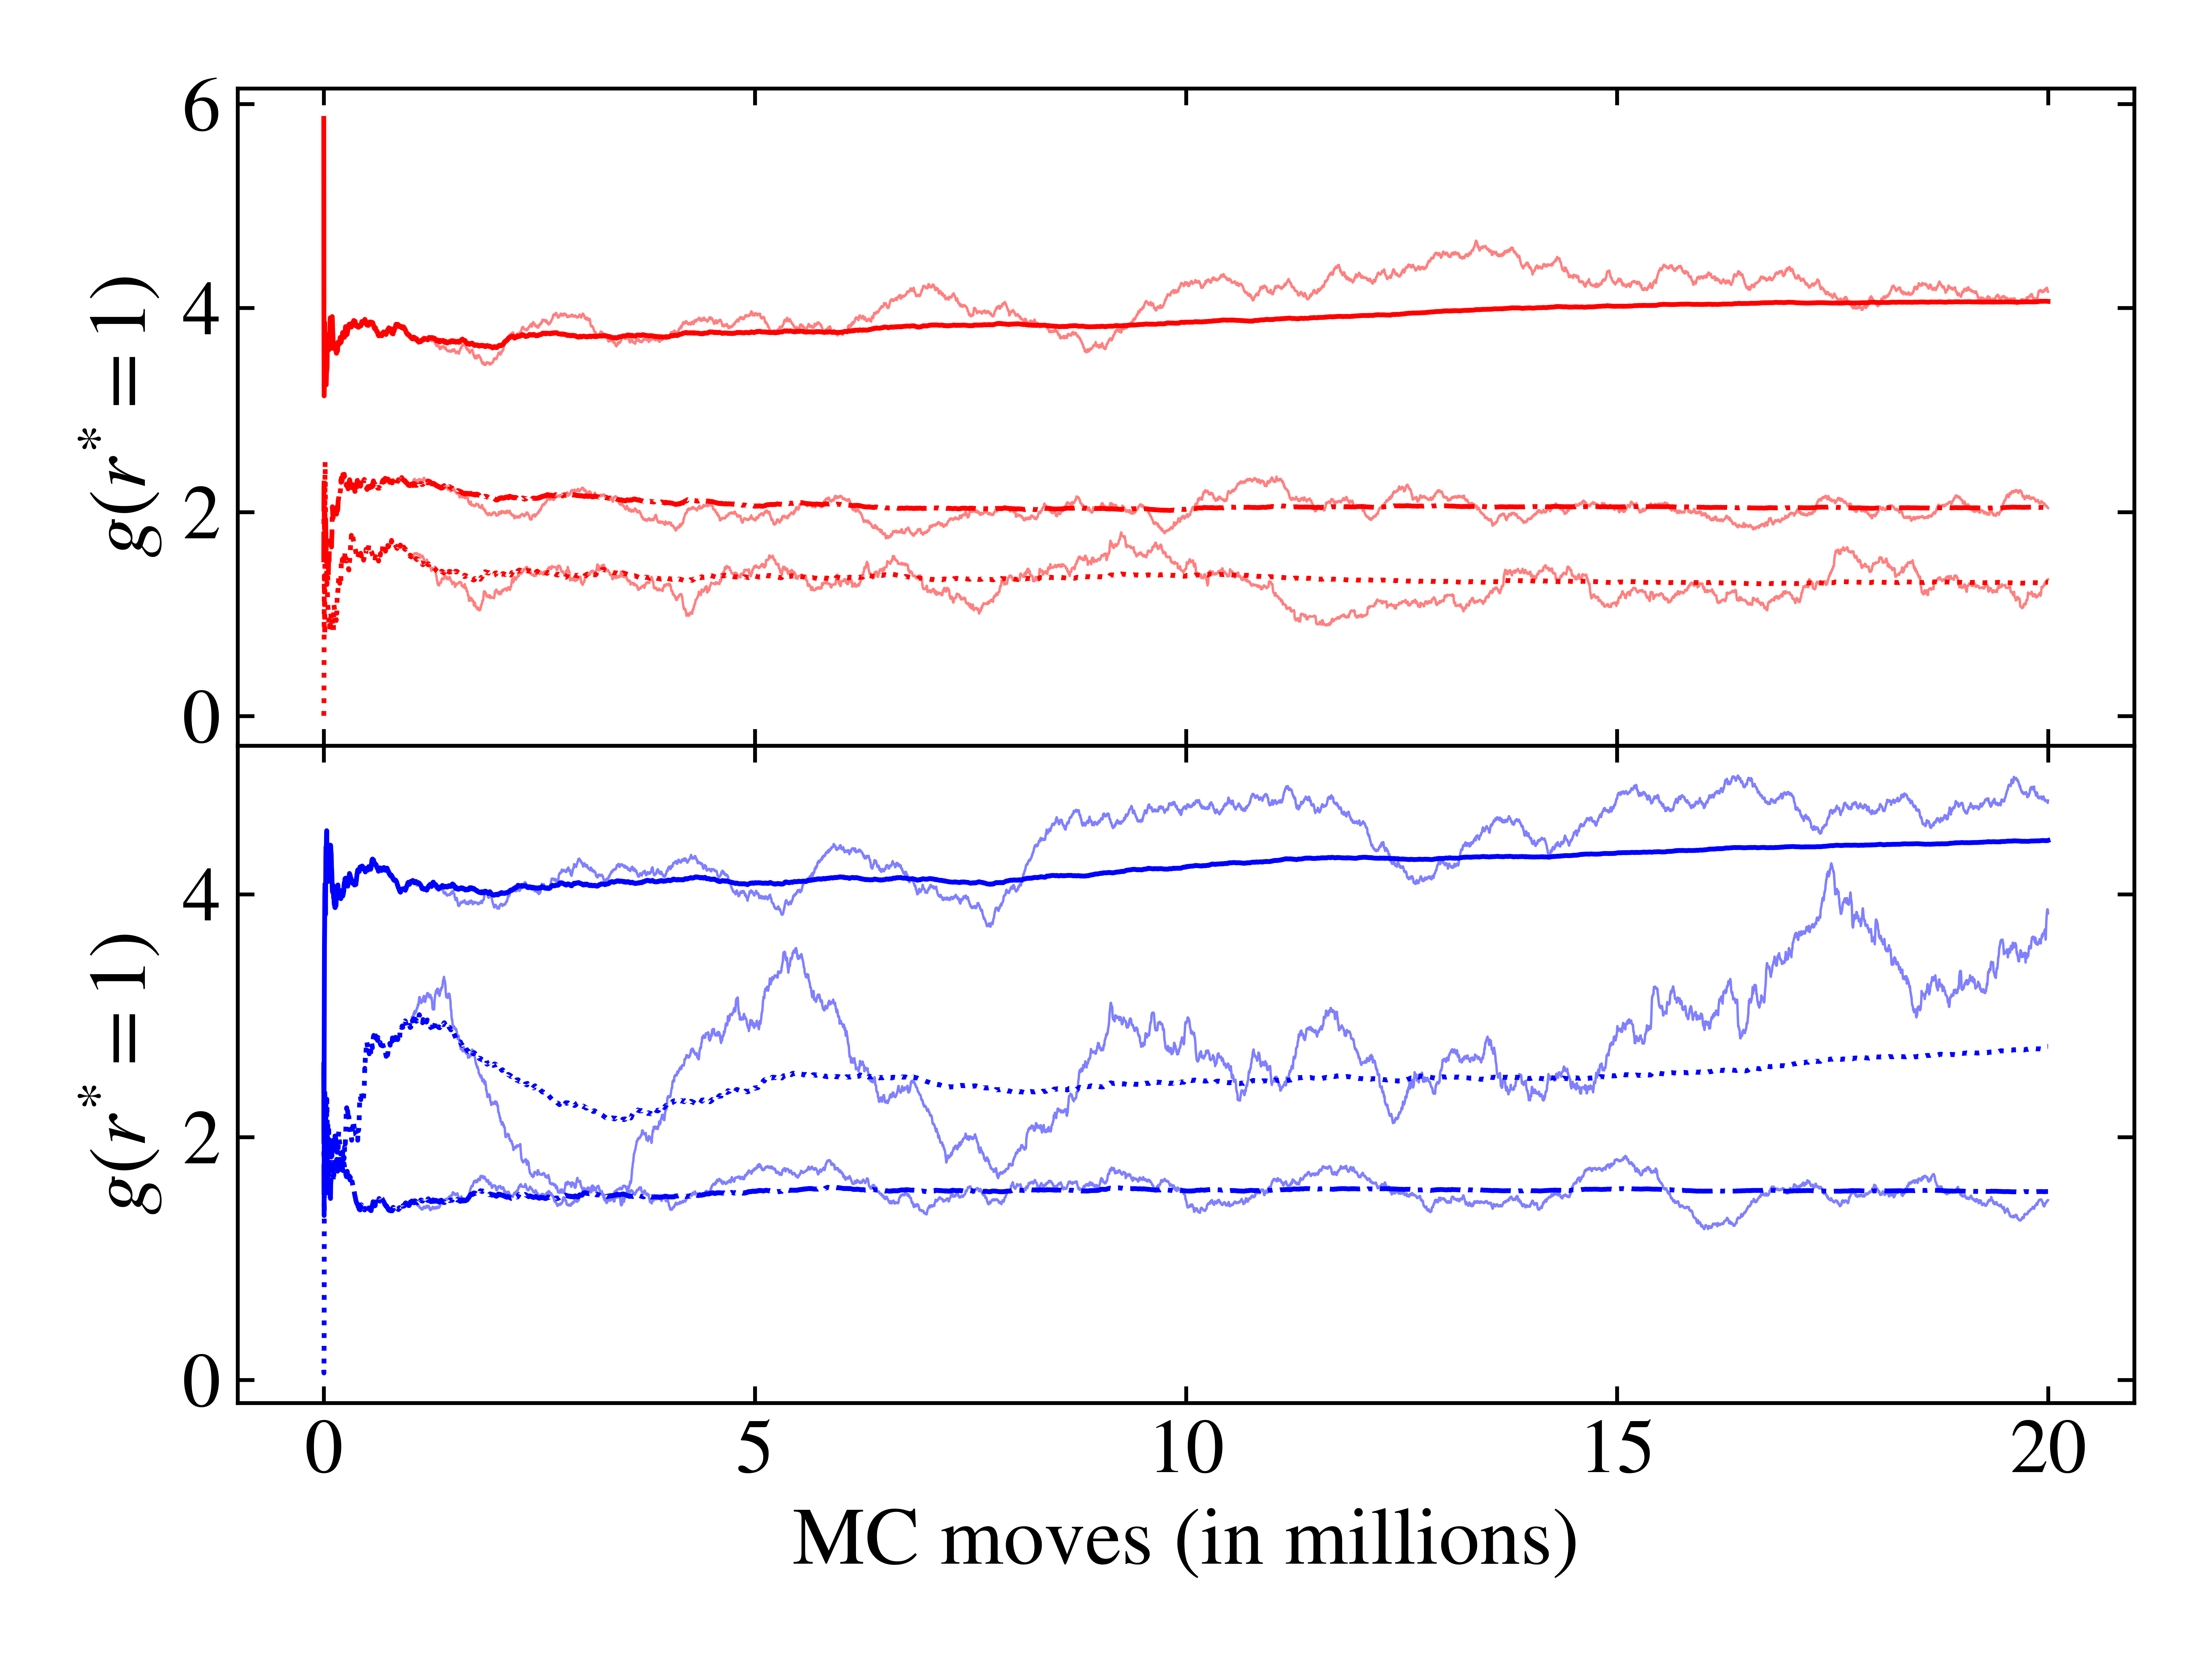
\includegraphics[width=\linewidth]{figures/convergence/gAtSigma_convergence.png}
	\caption{Typical convergence and fluctuation of the radial distribution function, $g(r^{*})$ evaluated at $r^{*}=1$. The smoother, darker lines show the variation of the cumulative average with increasing numbers of MC moves and are plotted for densities $\rho^{*} = 0.3, 0.8, 1.3$ represented by dotted, dash-dot, solid lines respectively. The lighter, jagged lines at any given point give a values of $g(r^{*}=1)$ averaged over the preceding 1 million MC moves. These are shown for isotherms $T^{*} = 0.75, 1.5$ represented by blue and red lines respectively. 
	}
	\label{fig:convergence}
\end{figure}

Graphs showing the convergence of the radial distribution function evaluated at $r^{*}=1$ and the fluctuation of a moving average over a fixed number of configurations for densities $\rho{}^{*}=0.3, 0.8, 1.3$ along isotherms $T^{*} = 0.75, 1.5$ are given in figure \ref{fig:convergence}. Ideally, we would have investigated the convergences of $u^{*}$ and $p^{*}$ however this would have required unduly amounts of computation time and the convergence $g(r^{*}=1)$ was chosen as a proxy for measuring the convergence of $g(r^{*})$ and thus $u^{*}$ and $p^{*}$.
These convergences are shown after the system had been equilibrated from its initial FCC configuration over \num{20e6} moves.
Along the isotherm $T^{*}=1.5$ the two lower density systems, $\rho{}^{*}=0.3, 0.8$, are observed to converge quite quickly, over approximately \num{2.5e6} moves with fluctuations of approximately $\pm{}10\%, 15\%$ respectively over the remaining moves. The system at $\rho{}^{*}=1.3$ seems to have initially converged quickly much like the lower density systems before starting to slowly rise after approximately \num{8e6} moves, evidenced by the fluctuations being distributed mostly around and then above the cumulative average in the two regions.
A similar trend is present in the system at $\rho{}^{*}=1.3$ along the isotherm $T^{*}=0.75$. Thus $g(r^{*}=1)$ is most likely underestimated in our high-density systems which, if it extends to $g(r^{*})$ for all $r^{*}$, \textit{could potentially account for the reduced $u^{*}$ and $p^{*}$ of our results when compared to those of NIST and Johnson et al}.
Convergence of the system at $T^{*}=0.75$, $\rho{}^{*}=0.8$ comparable to convergence at the same density along the higher isotherm, occurring over approximately \num{2.5e6} moves with fluctuations of $\pm{}10\%$.
Convergence of the system at $T^{*}=0.75$, $\rho{}^{*}=0.3$ shows qualitative characteristics not present in any of the other systems. First, the convergence of $g(r^{*}=1)$ displays some oscillatory behaviour which appears to stop at \num{10e6} moves. Fluctuations are then present fairly close to the cumulative average until \num{15e6} moves at which point $g(r^{*}=1)$ starts to increase. Without further investigation we are unable to comment on whether this increase continues past \num{20e6} moves. Thirdly, it is noted that $g(r^{*}=1)$ for $\rho{}^{*}=0.3$ converges to a higher value than for $\rho{}^{*}=0.8$. Since $g(r^{*}=1)$ can be interpreted as a measure of the likelihood of finding a particle a distance $r^{*}=1$ away from a reference particle, this would seemingly imply that particles in the lower density state are more tightly packed than particles in the higher density state \textit{- in contradiction to what you would expect.}
The trend of systems at very high densities being harder to converge has been shown by other workers \textbf{e.g. Wood \& Parker}.





\begin{figure}
	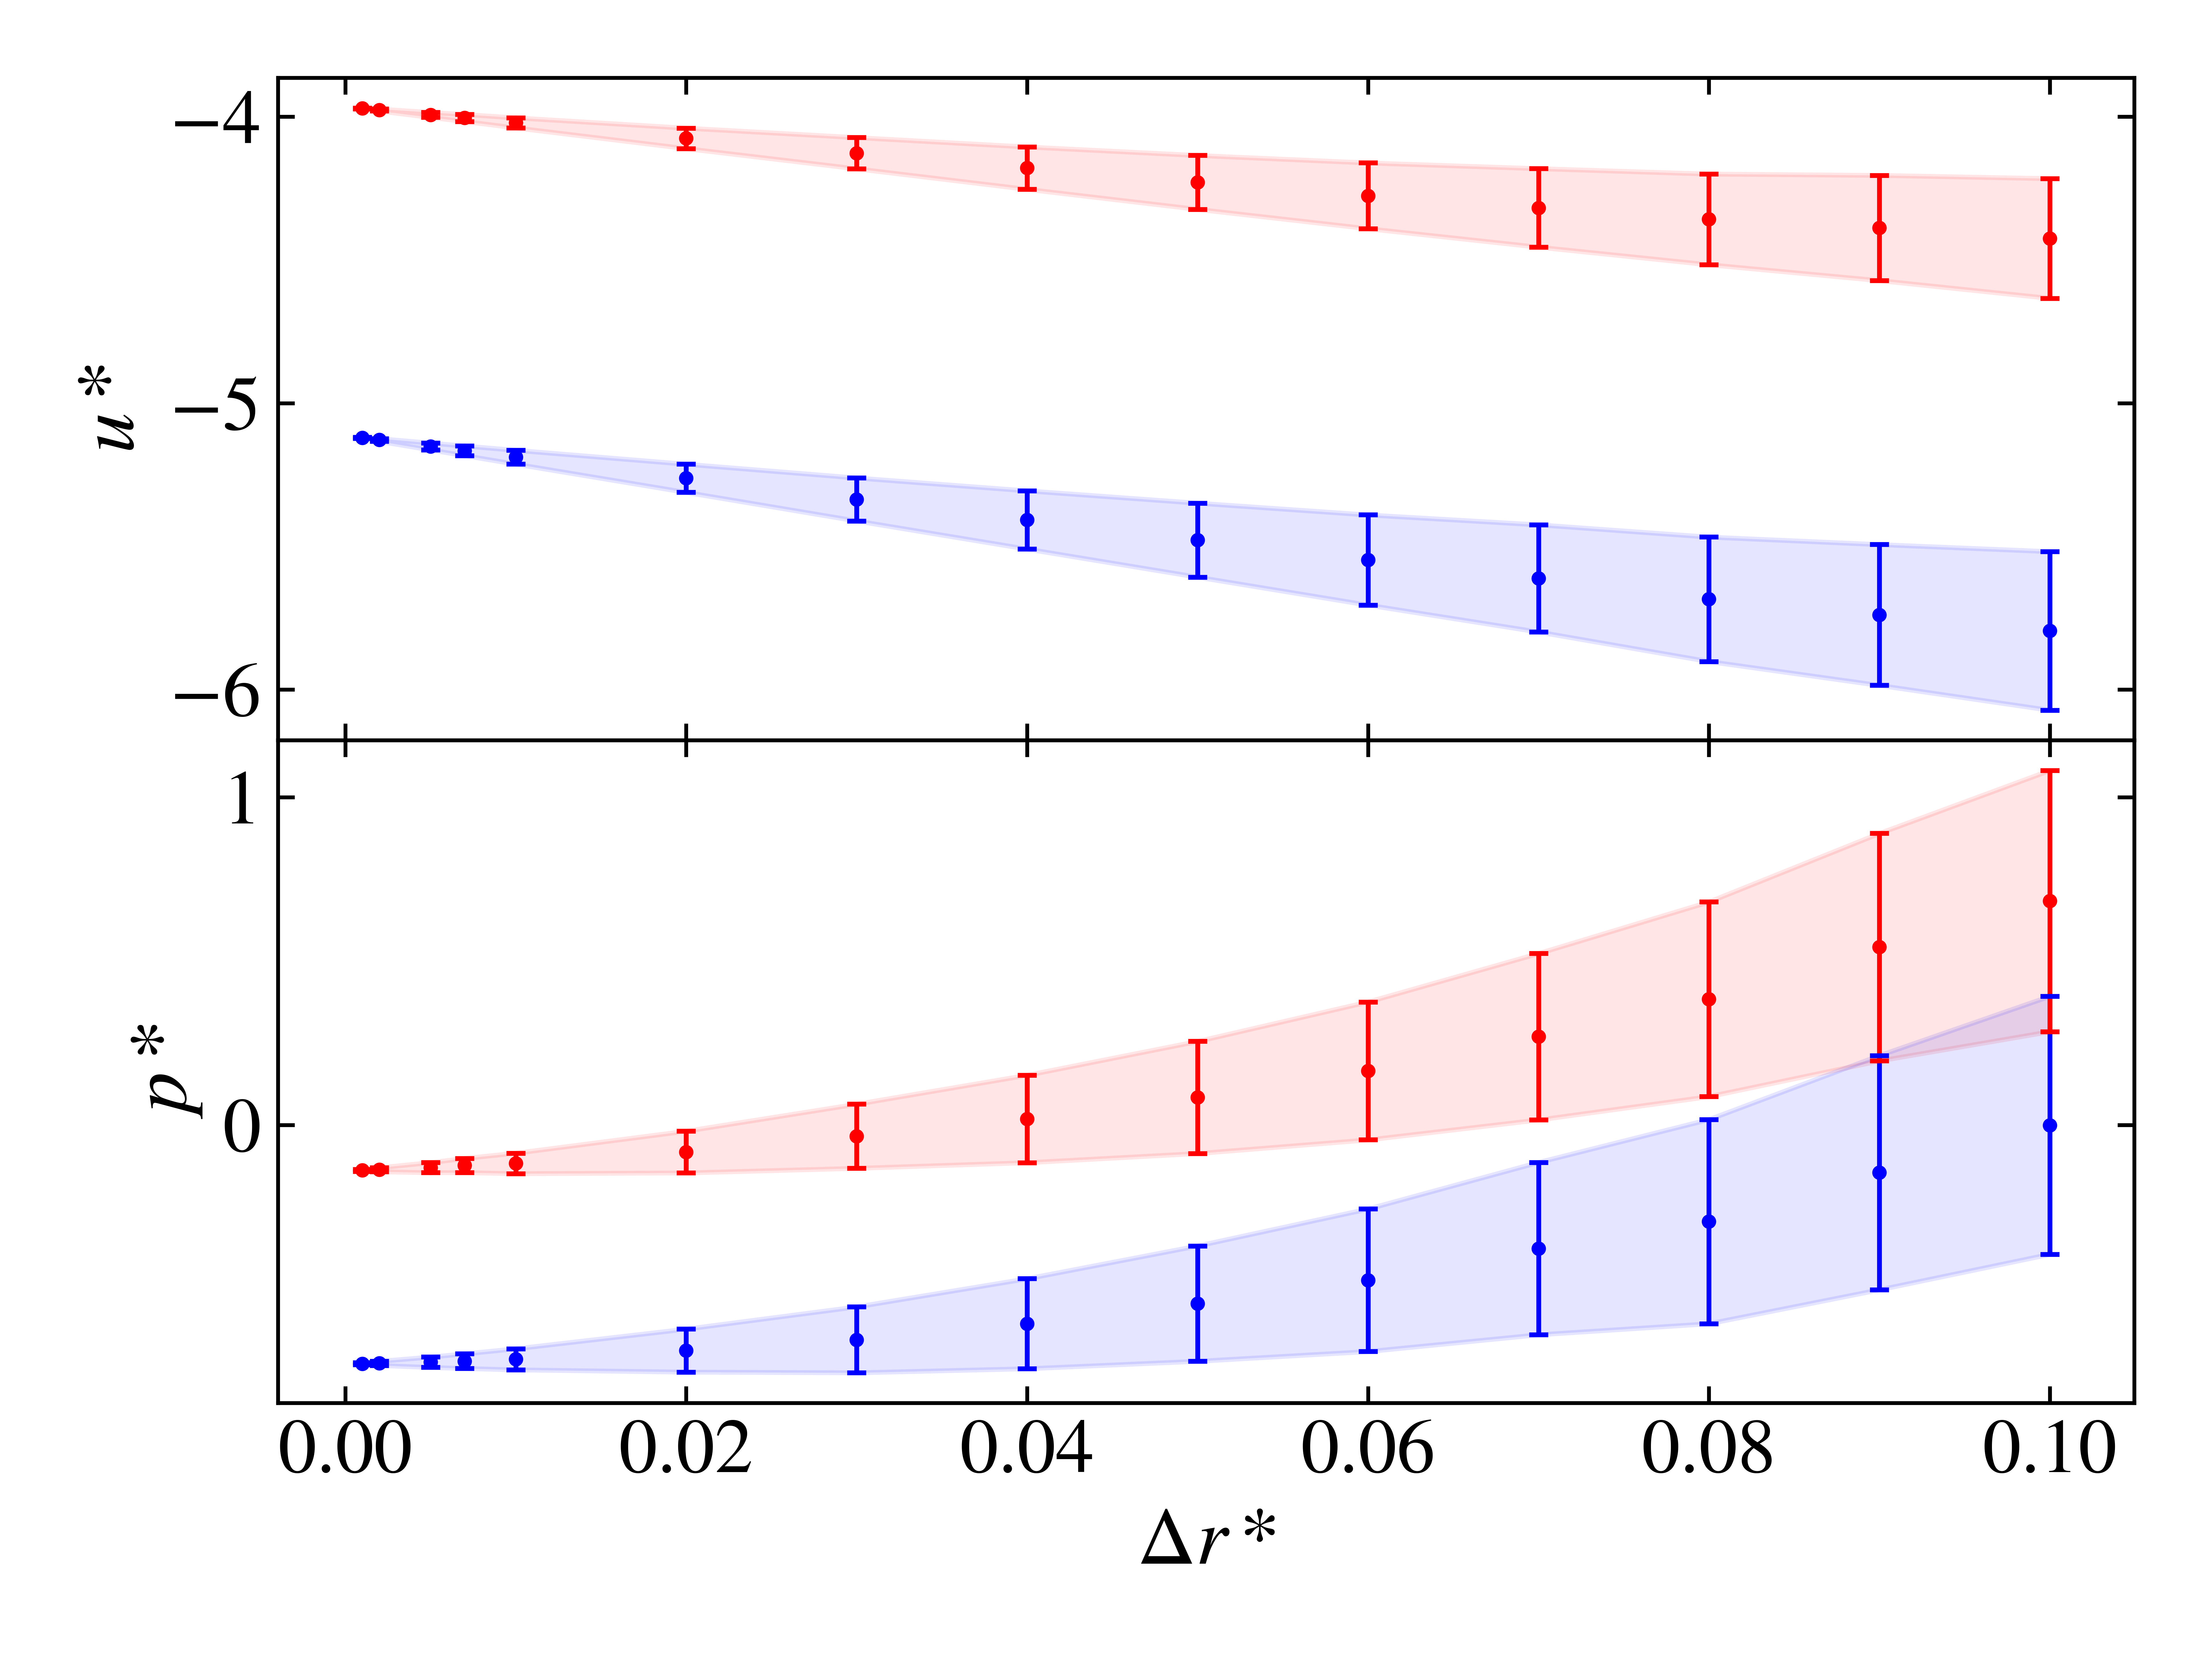
\includegraphics[width=\linewidth]{figures/binWidth/BWFeffect.png}
	\caption{Excess energy per particle, $u^{*}$, and excess pressure, $p^{*}$, against step-size $\Delta{}r^{*}$ (see discussion regarding equations \ref{eq:energy}, \ref{eq:pressure} in section \ref{s:methods}) evaluated for a system of density $\rho{}^{*}=0.6$ along isotherms $T^{*}=0.75, 1.5$ represented by blue and red markers respectively. Error bars show the standard error of the mean. Blue and red shaded areas are drawn to illustrate the increase in standard error with increasing step-size.}
	\label{fig:BWF}
\end{figure}


The step-size, $\Delta{}r^{*}$, in the numerical calculation of equations \ref{eq:energy} and \ref{eq:pressure} is a quantity of interest and importance. The closer $\Delta{}r^{*}$ to being infinitesimal, the closer our Riemann sum approximation is to evaluating the actual integral, leading to a more accurate result. However, the cost to decreasing $\Delta{}r^{*}$ is that the number of steps over which we evolve our systems must increase in order to maintain convergence, leading to prohibitive computation times at very small $\Delta{}r^{*}$. In order to explore the effect varying $\Delta{}r^{*}$ has on our results, we calculated $u^{*}$ and $p^{*}$ for systems of density $\rho{}^{*}=0.6$ along isotherms $T^{*}=0.75, 1.5$ at fourteen step-sizes ranging from \num{0.001} to \num{0.1}. This is shown in figure \ref{fig:BWF}. $u^{*}$ and $p^{*}$ are observed to decrease and increase respectively with increasing $\Delta{}r^{*}$. The standard errors of $u^{*}$ and $p^{*}$ both increase with $\Delta{}r^{*}$. A step size of \num{0.02} was chosen so that computations could be completed in a reasonable amount of time, corresponding to an approximate \num{3}\% (percentage) decrease in $u^{*}$ and a \num{0.05} (absolute) increase in $p^{*}$ along both isotherms. We do not account for these effects in our results - further investigation into the temperature and density dependences of this effect would need to be investigated in order to do so.


The accuracy of our model and method were investigated by direct comparison to Monte Carlo results at liquid and vapour-like densities along isotherms $T^{*} = 0.85, 0.90$ published by the National Institute of Standards and Technology (NIST). NIST's results are for \num{500} particles whose LJ interaction had been truncated to $r_\text{c}^{*}=3$ with standard long range corrections applied to $u^{*}$ and $p^{*}$. NIST's systems were equilibrated over \num{5.0e7} moves and quantities calculated over \num{2.5e8} moves, i.e. by factors of \num{2.5} and \num{12.5} more than ours. The configuration sampling rate of NIST's computations is not specified \textbf{ref NIST}.
Figure \ref{fig:NIST_u} shows $u^{*}$ from our simulations and NIST's data. With the exception of a single system, our values of $u^{*}$ are consistently reduced by \num{2} to \num{3}\% when compared the NIST data. This could be entirely attributed to the approximate \num{3}\% decrease found due to the Riemann sum approximation made in computing $u^{*}$ but this would need to be investigated further.
Figure \ref{fig:NIST_p} shows $p^{*}$ from our simulations and NIST's data. At vapour-like densities the absolute difference between our data and NIST's, $|\Delta{}p^{*}|$ increases linearly by a visual inspection. Our $p^{*}$ are observed to reduce below \num{0} with increasing density in this regime whereas NIST's results increase linearly with density by a visual inspection. At liquid-like densities, $\Delta{}p^{*}$ remains approximately constant at a value of about \num{-0.5}. This can not be accounted for by the effect of our approximation of equation \ref{eq:pressure} - in fact, it would place our values above those of NIST.
We find similar $\Delta{}u^{*}$ and $\Delta{}p^{*}$ when we compare our simulation to the extensive molecular dynamics results of Johnson et al \textbf{ref Johnson}. 

Mandel et al \textbf{ref Mandel: numerical solutions of the percus-yevick ...} found $p^{*}$ to be extremely sensitive to small errors in correlation functions such as $g(r^{*})$, much more so than the pressure. If the errors in $u^{*}$ can be attributed largely to approximations made in its calculation then it is likely that some small error in the production of $g(r^{*})$ is the cause of the discrepancies found in $p^{*}$. This is supported by the breakdown observed when computing $g(r^{*})$ at low temperature and densities as discussed above and illustrated in the lower panel of figure \ref{fig:convergence}.

\textbf{need to end discussion in a nicer way}



%\textit{The model and method were verified by direct comparison to Monte Carlo results at liquid and vapour-like densities along isotherms $T^{*}=0.85, 0.90$ published by United States' National Institute of Standard and Technology (NIST). NIST's results were for 500 particles whose Lennard-Jones interaction had been truncated to $3\sigma{}$ and standard long range corrections had been applied. Their systems were equilibrated for $5.0\text{e}7$ moves and quantities calculated over $2.5\text{e}8$ moves. Figure \ref{fig:NIST_comparison} shows the configuration energy per particle, $u^*$, and virial pressure, $p^{*} = P - \rho{}kT$ for both our system and NIST's. Our results were obtained as described in section \ref{s:methods}. See appendix \ref{a:NIST} for the values and their associated uncertainties of NIST's and our simulations.}


\begin{figure}
	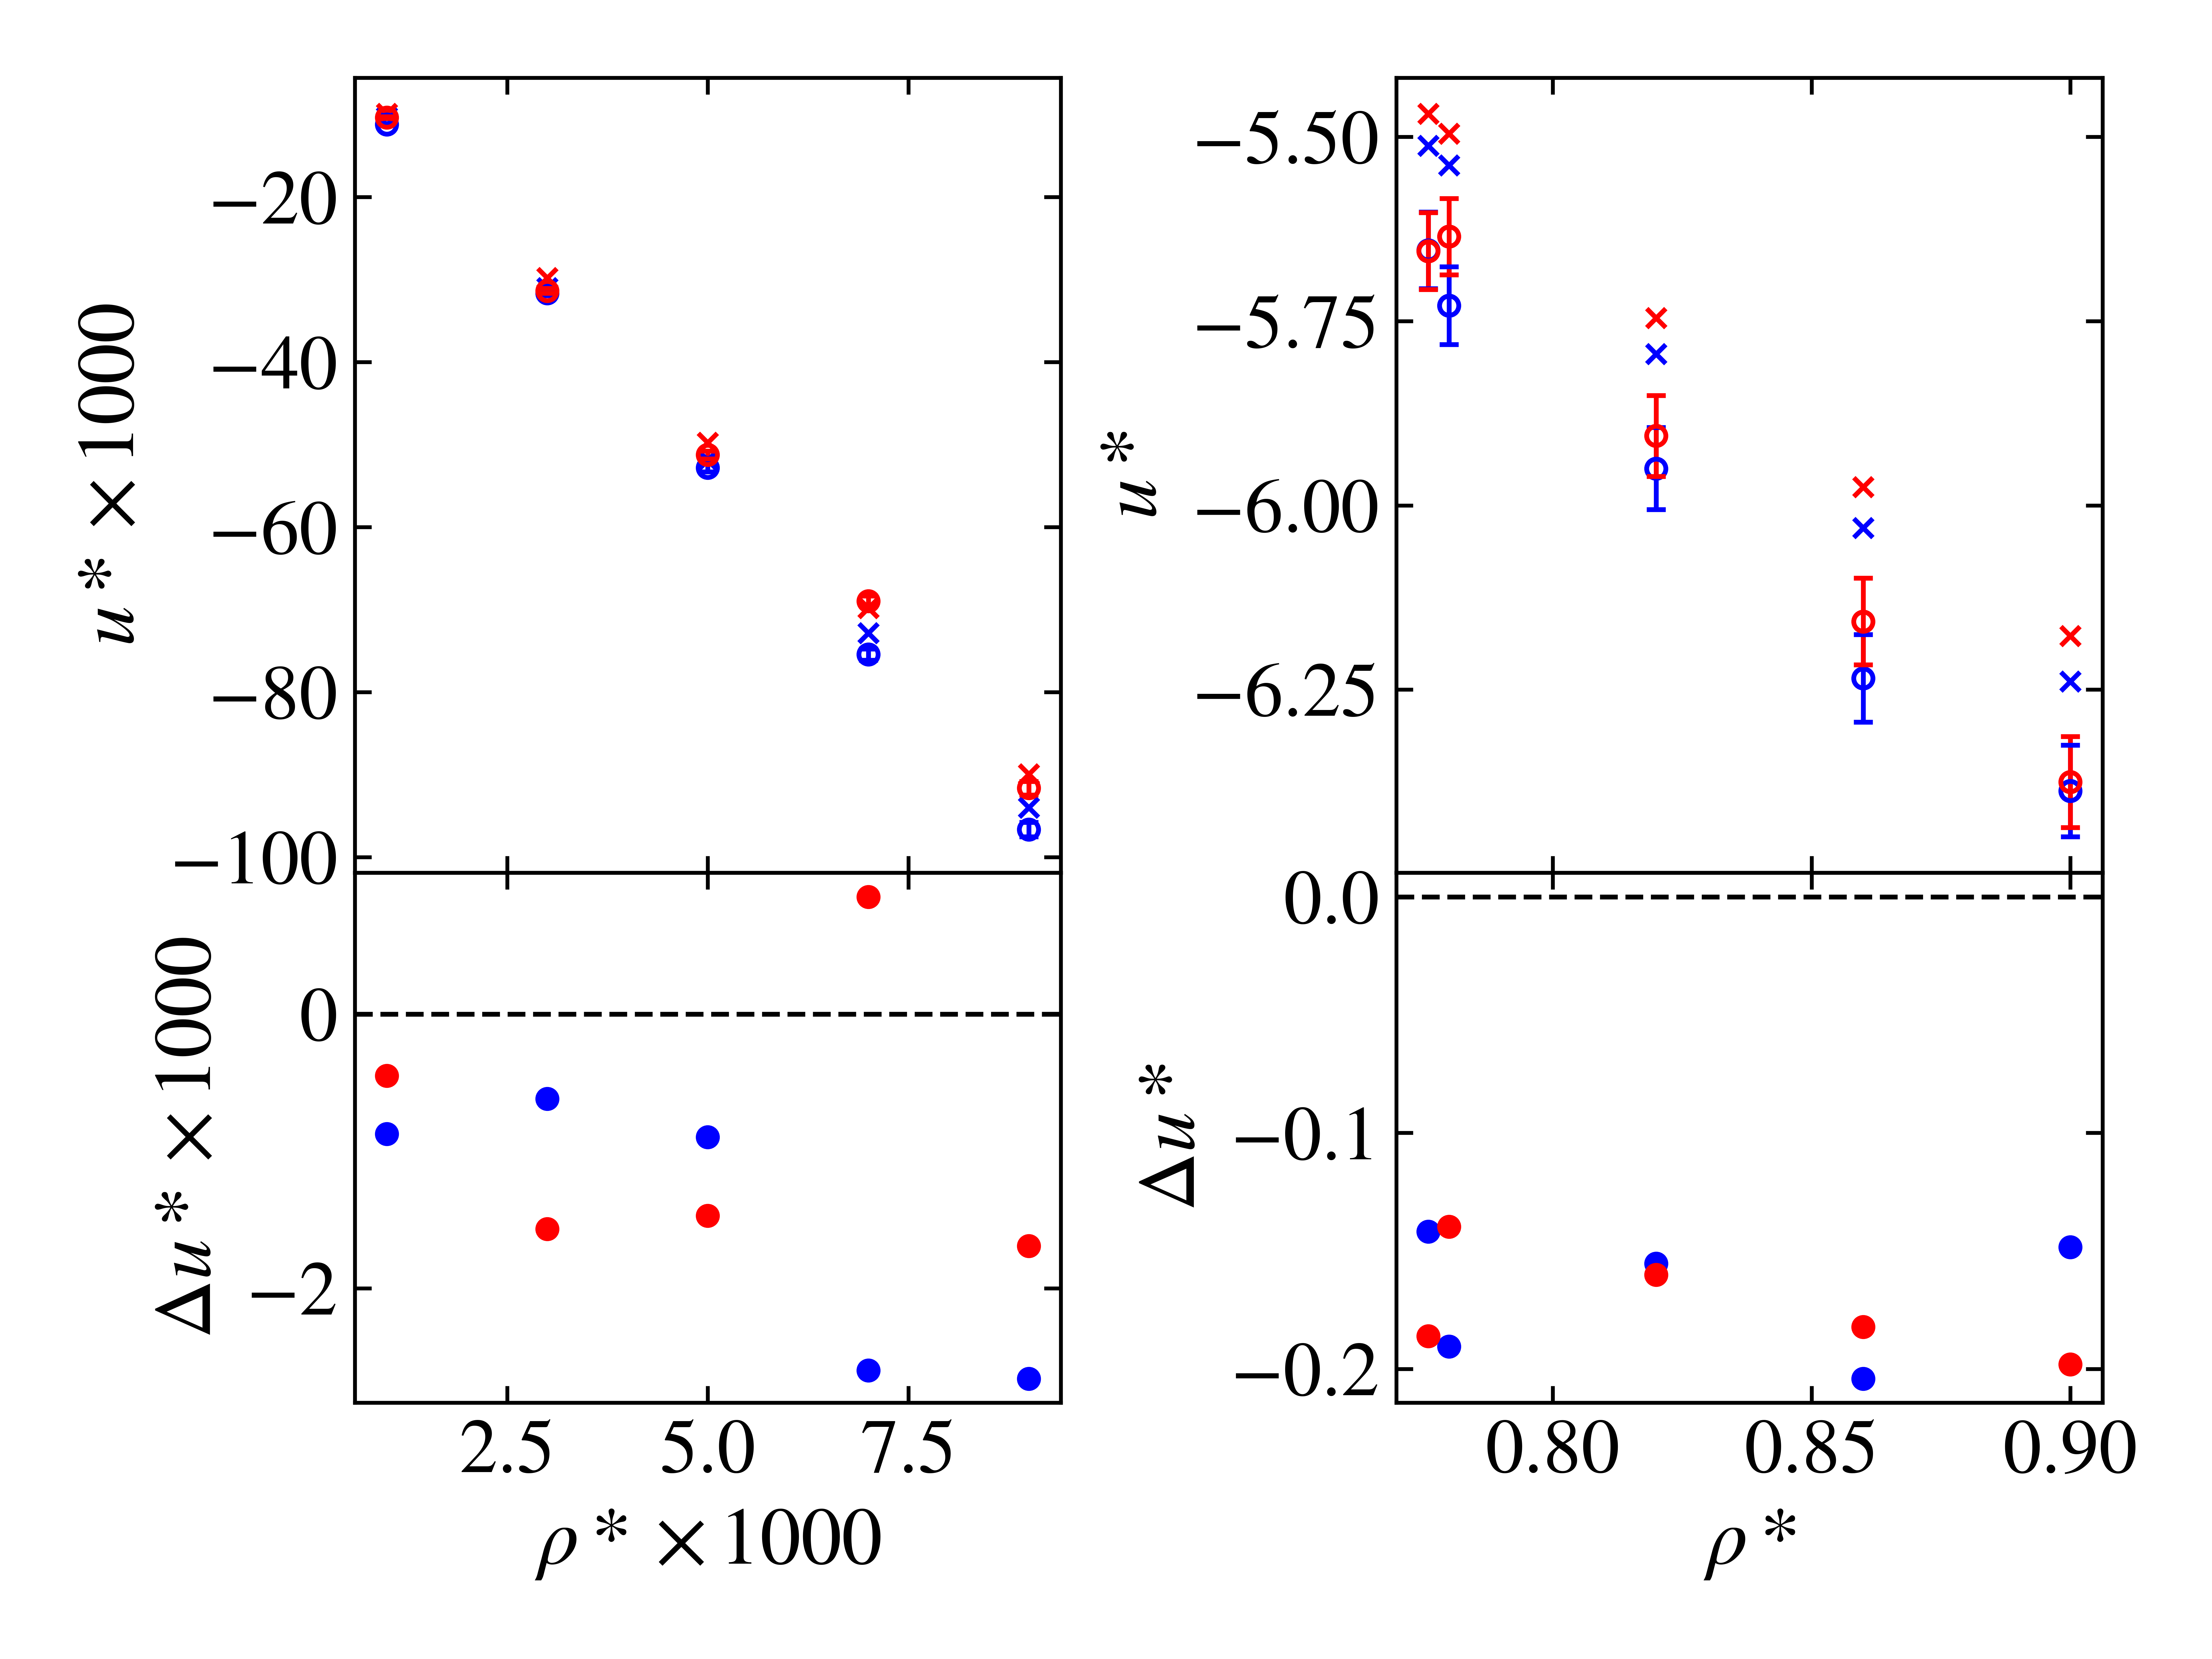
\includegraphics[width=\linewidth]{figures/NIST_comparison/NIST_u.png}
	\caption{Excess energy per particle, $u^{*}$, at vapour-like (upper-left panel) and liquid-like (upper-right panel) densities, $\rho{}^{*}$. Our MC results and those of the National Institute of Standards and Technology (NIST) are represented by unfilled circles and crosses respectively. Data is shown for isotherms $T^{*}=0.85, 0.90$ by blue and red markers respectively. Error bars for our MC data show the standard error of the mean. Error bars are not shown for NIST's data for visual clarity. The differences between our results and NIST's results, $\Delta{}u^{*} = u_\text{our}^{*} - u_\text{NIST}^{*}$ are shown in the lower panel. A dotted line has been added along $\Delta{}u^{*}=0$ for reference. Note that some values have been scaled by a factor of 1000.}
	\label{fig:NIST_u}
\end{figure}

\begin{figure}
	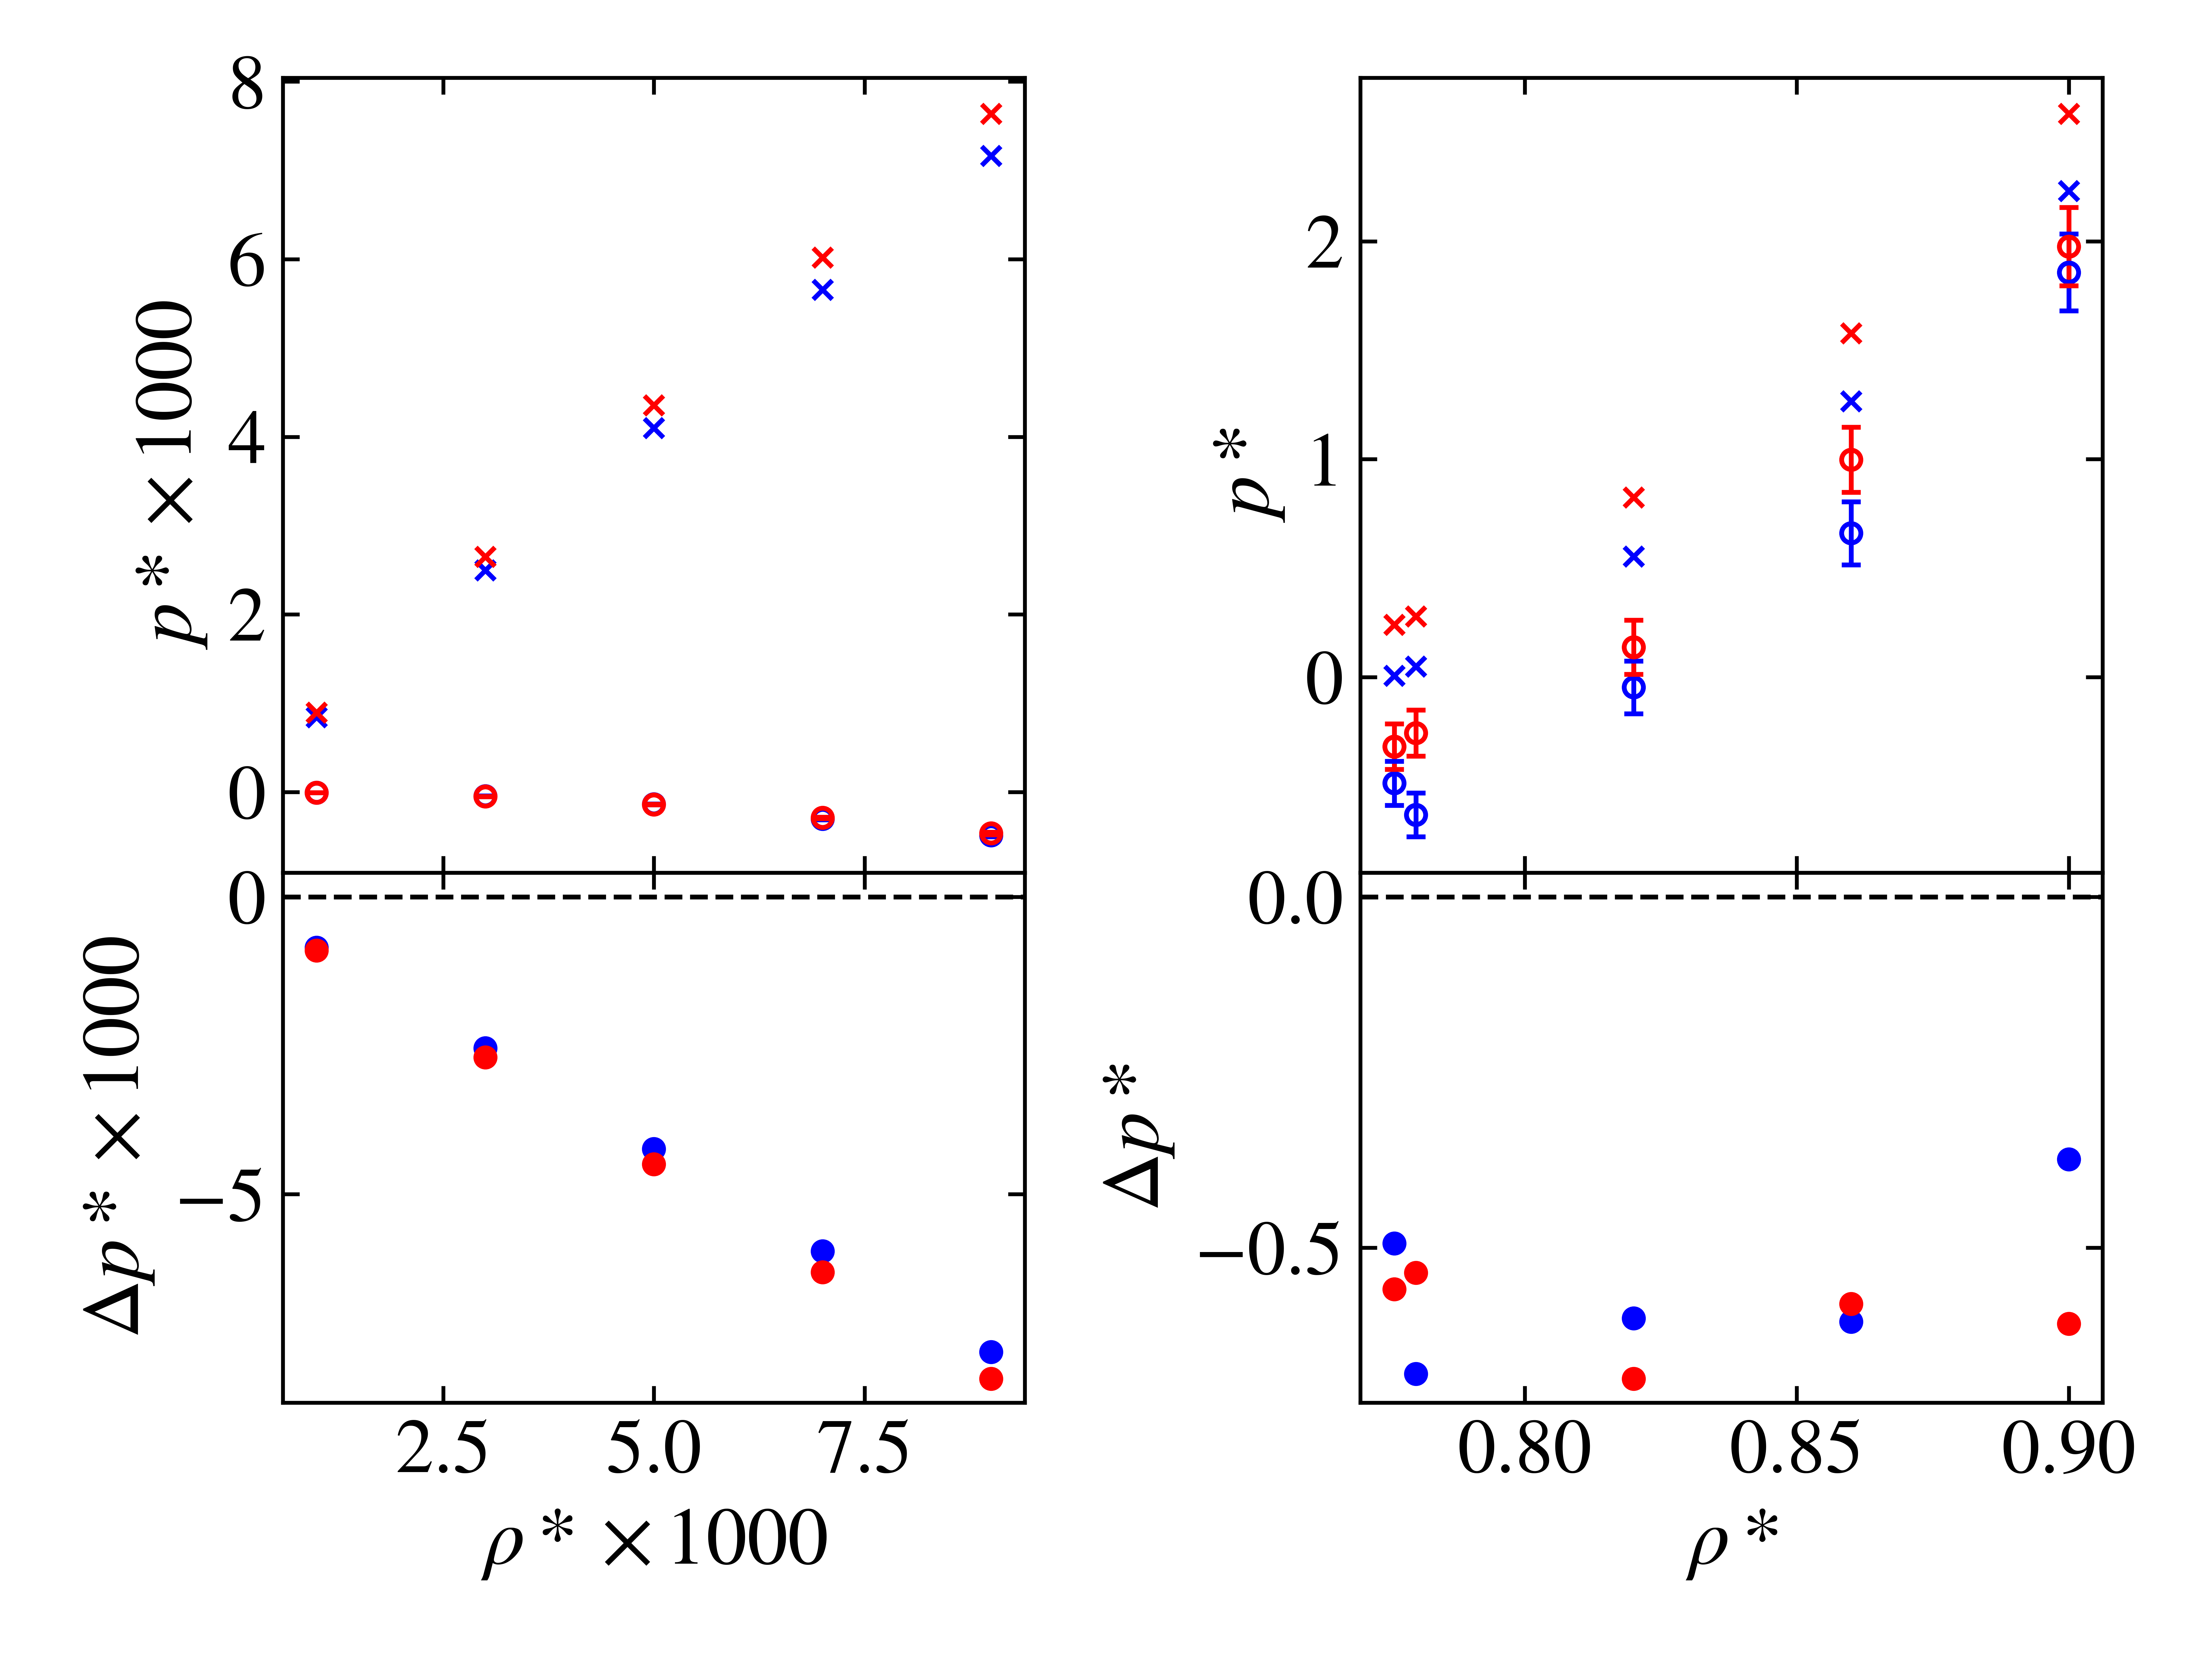
\includegraphics[width=\linewidth]{figures/NIST_comparison/NIST_p.png}
	\caption{Excess pressure, $p^{*}$, at vapour-like (upper-left panel, note that these values have been scaled by a factor of 1000) and liquid-like (upper-right panel) densities, $\rho{}^{*}$. Our MC results and those of the National Institute of Standards and Technology (NIST) are represented by unfilled circles and crosses respectively. Data is shown for isotherms $T^{*}=0.85, 0.90$ by blue and red markers respectively. Error bars for our MC data show the standard error of the mean. Error bars are not shown for NIST's data for visual clarity. The differences between our results and NIST's results, $\Delta{}p^{*} = p_\text{our}^{*} - p_\text{NIST}^{*}$ are shown in the lower panel. A dotted line has been added along $\Delta{}p^{*}=0$ for reference. Note that some values have been scaled by a factor of 1000.}
	\label{fig:NIST_p}
\end{figure}

%\section{Discussion} \label{s:analysis}
%\lipsum[1-15]



\section{Conclusions} \label{s:conclusions}
%\lipsum[1-5]

\begin{thebibliography}{}

%\bibitem{ref01} A. N. Other, Title of the Book, edition, publishers, place of publication (year of publication), p. 123.   % example reference



\bibitem{MC} N. Metropolis, et al., Equation of State Calculations by Fast Computing Machines, J. Chem. Phys. 21, 1087 (1953), doi:10.1063/1.1699114

\bibitem{SimpleLiquids} J. P. Hansen, I. R. McDonald, Theory of Simple Liquids, 3rd, Academic Press, Massachusetts (2006) \textbf{PAGE}

\bibitem{CompSimLiq} M. P. Allen, D. J. Tildesley, Computer Simulation of Liquids, 2nd, Oxford University Press, Oxford (2017) \textbf{PAGE}

\bibitem{HansenVerlet1} J. P. Hansen, L. Verlet, Phase Transitions of the Lennard-Jones System, Phys. Rev. 184, 151 (1969), doi:10.1103/PhysRev.184.151

\bibitem{Hansen2} J. P. Hansen, Phase Transition of the Lennard-Jones System. II. High-Temperature Limit, Phys. Rev. A 2, 221 (1970), doi:10.1103/PhysRevA.2.221

\bibitem{MandelEtAl} F. Mandel, et al., Numerical Solutions of the Percus-Yevick Equation for the Lennard-Jones (6-12) and Hard-Sphere Potentials, J. Chem. Phys. 52, 3315 (1970), doi:10.1063/1.1673491

\bibitem{WoodParker} W. W. Wood, F. R. Parker, Monte Carlo Equation of State of Molecules Interacting with the Lennard-Jones Potential. I. A Supercritical Isotherm at about Twice the Critical Temperature, J. Chem. Phys. 27, 720 (1957), doi:10.1063/1.1743822

\bibitem{NIST} Published data for testing codes: Lennard-Jones Fluid Properties, National Institute of Standards and Technology, accessed 17 Feb 2020, available at: https://www.nist.gov/mml/csd/chemical-informatics-research-group/lennard-jones-fluid-properties

\bibitem{Ree} F. H. Ree, Analytic representation of thermodynamic data for the
Lennard-Jones fluid, J. Chem. Phys. 73, 5401 (1980), doi:10.1063/1.439940

\bibitem{Johnson} J. K. Johnson,The Lennard-Jones equation of state revisited , Mol. Phys. 78:3, 591-618 (1993), doi:10.1080/00268979300100411

\bibitem{errors}I. G. Hughes, T. P. A Hase, Measurements and their Uncertainties A Practical Guide to Modern Error Analysis, 1st, Oxford University Press, Oxford (2010)

\end{thebibliography} 

%\clearpage
%\appendix
%\section{Error Analysis} \label{a:errors}
%All propagation of errors is performed as outlined in \cite{errors}.
%
%\clearpage
%\section{Comparison to NIST data} \label{a:NIST}
%
%
%% Please add the following required packages to your document preamble:
%% \usepackage{booktabs}
%% \usepackage{multirow}
%% \usepackage{graphicx}
%\begin{table}[]
%	\resizebox{\textwidth}{!}{%
%		\begin{tabular}{@{}rrrrrrrrrr@{}}
%			\toprule
%			$T^*$                  & $\rho{}^*$ & $U_\text{NIST}^*$ & $\pm$    & $U_\text{ours}^*$ & $\pm$   & $p_\text{NIST}^*$ & $\pm$    & $p_\text{ours}^*$ & $\pm$   \\ \midrule
%			\multirow{10}{*}{0.85} & 1.00E-3    & -1.0317E-2       & 2.34E-5 & -9.968E-3         & 9.17E-5 & 8.4402E-4        & 4.66E-8 & -5.288E-6         & 1.72E-7 \\
%			& 3.00E-3    & -3.1019E-2       & 5.91E-5 & -3.156E-2         & 2.87E-4 & 2.4965E-3        & 4.99E-7 & -6.121E-5         & 1.48E-6 \\
%			& 5.00E-3   & -5.1901E-2       & 7.53E-5 & -5.485E-2         & 5 .07E-4 & 4.1003E-3        & 5.05E-7 & -1.472E-4         & 4.75E-6 \\
%			& 7.00E-3   & -7.2834E-2       & 1.34E-4 & -7.499E-2         & 6.87E-4 & 5.6565E-3        & 7.96E-7 & -2.854E-4         & 8.98E-6 \\
%			& 9.00E-3   & -9.3973E-2       & 1.29E-4 & -9.863E-2         & 9.18E-4 & 7.1641E-3        & 2.24E-6 & -4.568E-4         & 1.51E-5 \\
%			& 7.76E-1   & -5.5121       & 4.55E-4 & -5.623            & 5.21E-2 & 6.7714E-3        & 1.77E-3 & -5.577E-1         & 9.91E-2 \\
%			& 7.80E-1   & -5.5386       & 7.26E-4 & -5.611            & 5.14E-2 & 4.7924E-2        & 3.18E-3 & -6.311E-1         & 9.88E-2 \\
%			& 8.20E-1   & -5.7947       & 6.03E-4 & -5.908            & 5.59E-2 & 5.5355E-1        & 4.13E-3 & 2.588E-1          & 1.25E-1 \\
%			& 8.60E-1   & -6.0305       & 2.38E-3 & -6.175            & 5.87E-2 & 1.2660        & 1.36E-2 & 4.973E-1          & 1.41E-1 \\
%			& 9.00E-1   & -6.2391       & 5.27E-3 & -6.346            & 6.17E-2 & 2.2314        & 2.72E-2 & 1.823             & 1.75E-1 \\ \cmidrule(lr){1-10}
%			\multirow{10}{*}{0.90} & 1.00E-3   & -9.9165E-3       & 1.89E-5 & -9.989E-3         & 9.05E-5 & 8.9429E-4        & 2.48E-8 & -6.475E-6         & 1.76E-7 \\
%			& 3.00E-3   & -2.9787E-2       & 3.21E-5 & -3.065E-2         & 2.79E-4 & 2.6485E-3        & 2.54E-7 & -4.368E-5         & 1.70E-6 \\
%			& 5.00E-3   & -4.9771E-2       & 3.80E-5 & -5.226E-2         & 4.75E-4 & 4.3569E-3        & 2.19E-7 & -1.426E-4         & 4.35E-6 \\
%			& 7.00E-3   & -6.9805E-2       & 7.66E-5 & 7.179E-2          & 6.50E-4 & 6.0193E-3        & 1.02E-6 & -3.075E-4         & 8.14E-6 \\
%			& 9.00E-3   & -8.9936E-2       & 2.44E-5 & -9.151E-2         & 8.33E-4 & 7.6363E-3        & 1.44E-6 & -4.295E-4         & 1.41E-5 \\
%			& 7.76E-1   & -5.4689       & 4.20E-4 & -5.615            & 5.21E-2 & 2.4056E-1        & 2.74E-3 & -2.486E-1         & 1.04E-1 \\
%			& 7.80E-1   & -5.4956       & 7.86E-4 & -5.627            & 5.20E-2 & 2.7851E-1        & 2.97E-3 & -2.576E-1         & 1.06E-1 \\
%			& 8.20E-1   & -5.7456       & 7.51E-4 & -5.870            & 5.53E-2 & 8.2386E-1        & 2.85E-3 & 2.921E-1          & 1.25E-1 \\
%			& 8.60E-1   & -5.9753       & 5.53E-4 & -6.130            & 5.89E-2 & 1.5781        & 3.29E-3 & 1.193             & 1.53E-1 \\
%			& 9.00E-1   & -6.1773       & 1.57E-3 & -6.312            & 6.14E-2 & 2.5848        & 9.54E-3 & 1.871             & 1.75E-1 \\ \bottomrule
%		\end{tabular}%
%	}
%\end{table}

\end{document}